% TODO: Gendern?
% TODO: README.md schreiben (Sollte Details zu DNS config enthalten)
\documentclass[11pt,a4paper]{article}
\usepackage[utf8]{inputenc}
\usepackage[T1]{fontenc}
\usepackage{lmodern}
\usepackage[ngerman]{babel}
\usepackage{graphicx}
% \usepackage{babelbib}
\usepackage{hologo}
\usepackage{csquotes}
\usepackage{amsmath}
\usepackage{amssymb}
\usepackage{amsthm}
\usepackage{biblatex}
\usepackage{listings}
\usepackage{xcolor}
\lstset{basicstyle=\ttfamily}
\addbibresource{literature.bib}


\definecolor{codegreen}{rgb}{0,0.6,0}
\definecolor{codegray}{rgb}{0.5,0.5,0.5}
\definecolor{codepurple}{rgb}{0.58,0,0.82}
\definecolor{backcolour}{rgb}{0.95,0.95,0.92}

\lstdefinestyle{mystyle}{
    backgroundcolor=\color{backcolour},   
    commentstyle=\color{codegreen},
    keywordstyle=\color{magenta},
    numberstyle=\tiny\color{codegray},
    stringstyle=\color{codepurple},
    basicstyle=\ttfamily\footnotesize,
    breakatwhitespace=false,         
    breaklines=true,                 
    captionpos=b,                    
    keepspaces=true,                 
    numbers=left,                    
    numbersep=5pt,                  
    showspaces=false,                
    showstringspaces=false,
    showtabs=false,                  
    tabsize=2
}

\lstset{style=mystyle}
\hyphenation{In-stand-setz-ungs-kon-fi-gu-ra-tio-nen}
\hyphenation{Name-spaces}

\begin{document}

\tableofcontents

\section{Zusammenfassung}
Kubernetes bietet als weit verbreitetes Container-Orchestrierungs-Tool vielfältige Möglichkeiten.
Diese Arbeit ordnet Kubernetes und die zugrundeliegende Motivation in einen historischen Kontext ein. 
Darauf aufbauend werden wichtige Komponenten und deren Verwendung beschrieben und erklärt.
Zur Illustration wird ein Anwendungsfall aus dem Bereich des Data Farmings verwendet, 
bei dem ein Simulationsmodell zur Optimierung der Einsatzbereitschaft einer Fahrzeugflotte mit den 
durch Kubernetes zur Verfügung gestellten Komponenten skalierbar betrieben wird. Dieses Simulationsmodell
gliedert sich in eine Microservice-Architektur ein, die Bedienung und Auswertung der Simulation erlaubt, 
sowie Mittel zur Speicherung von Konfigurationen und Ergebnissen bietet.
Im Ergebnis zeigt sich Kubernetes als geeignet, um sowohl die Simulation als auch die notwendigen 
Stützservices skalierbar zu betreiben.
Dennoch werden auch Limitationen diskutiert, die zum Teil durch fehlende 
Hardware-Ressourcen aber auch durch die Komplexität von Kubernetes entstehen können.
Abschließend folgt ein Ausblick über die mögliche Weiterentwicklung des Anwendungsfalls
an sich und die zu erwartende Entwicklung von Kubernetes im Allgemeinen in den nächsten Jahren.



\section{Einleitung}
\label{sec:einleitung}
Die vorliegende Arbeit soll einen Überblick über das Container-\linebreak Orchestrierungs-Tool \emph{Kubernetes} geben. 
Dazu werden zunächst Historie und grundlegende Funktionsprinzipien von Kubernetes beschrieben, die anschließend
anhand einer beispielhaften Anwendung aus dem Bereich verteilter, agentenbasierter Simulationen demonstriert werden.

Zunächst soll die Historie betrachtet werden, vor deren Hintergrund Kubernetes entstanden ist.
Das stetige Ziel, das in sich durch diese Historie zieht, ist das Bereitstellen von Applikationen.
Kominos et al. \cite{7899247} beschreiben die 1960er Jahre als Ursprung des Cloud-Computings.
Zu dieser Zeit liefen Applikationen oft auf einer gemeinsamen Hardware und die Ressourcenverteilung erfolgte unmittelbar durch das zugrundeliegende Betriebssystem.
Ein derartiges Szenario (auch als „Bare-Metal“ bezeichnet) bringt in der Regel mehrere Herausforderungen mit sich.
Zum einen kann es schnell zu Abhängigkeitskonflikten zwischen den verschiedenen Applikationen geben.
Ist eine Applikation darauf angewiesen eine bestimmte Abhängigkeit in der Version <1.4 zu nutzen und eine andere
benötigt eine Version \(\geq 1.4\) derselben Abhängigkeit, lässt sich das nur schwer vereinbaren.
Zum anderen erschwert dieser Aufbau eine effiziente Ressourcenverteilung. Selbst wenn eine Applikation alleine auf einem Rechner betrieben wird (z.B. um Konflikte zu anderen
Applikationen zu vermeiden), muss dieser Rechner ausreichende Kapazitäten haben, um die höchsten Anfragespitzen an diese Applikation zu verarbeiten.
Selbst dann, wenn diese Anfragespitzen nur äußerst selten erreicht werden.

Eine Weiterentwicklung dieser Bare-Metal-Architektur waren virtuelle Maschinen. Virtuelle Maschinen erlauben es, auf derselben Hardware mehrere virtuelle Instanzen eines
Systems zu nutzen. Die Instanzen nutzen dabei nicht direkt die physischen Ressourcen, sondern lediglich virtuelle, die durch Software nachgebildet werden \cite{kofler2021docker}.
Dadurch, dass verschiedene Applikationen in verschiedenen virtuellen Maschinen betrieben werden, können Abhängigkeitskonflikte zwischen Applikationen
vermieden werden. Weiterhin sind virtuelle Maschinen leichter auszubringen und zu administrieren als Bare-Metal-Lösungen.
Grundsätzlich können mit diesem Ansatz Applikationen auch flexibler und skalierbarer bereitgestellt werden.
Leistungsfähige Hardware kann Anfragespitzen einer Applikation in einer virtuellen Maschine abfangen und zu anderen Zeiten anderen virtuellen Maschinen mit anderen
Applikationen diese Ressourcen zuweisen.
Obwohl das schon einige Verbesserungen im Vergleich zu Bare-Metal-Lösungen sind, haben auch virtuelle Maschinen ihre eigenen Limitationen.
Da virtuelle Maschinen jeweils Ressourcen für ein eigenes Betriebssystem beanspruchen, geht vergleichsweise viel Leistung verloren, 
die besser in der Applikation genutzt werden könnte.

Die nächste Stufe der Weiterentwicklung waren (Software-)Container. Container haben einige Gemeinsamkeiten mit virtuellen Maschinen, doch der wesentliche Unterschied ist,
dass Container deutlich leichtgewichtiger sind. Das wird unter anderem dadurch erreicht, dass sie statt ein komplett eigenes Betriebssystem zu verwenden, 
Anteile des Host-Betriebssystems mitnutzen. Dadurch sind die „Baupläne“ (sog. Images) für Container im Allgemeinen kleiner als für klassische virtuelle Maschinen.
Durch den verringerten Overhead können auf gleicher Hardware auch mehr Container parallel betrieben werden, als es mit virtuellen Maschinen möglich wäre.
Durch diesen Umstand und dadurch, dass Container meist innerhalb weniger Sekunden gestartet werden können, sind diese besonders geeignet,
um flexibel auf unterschiedliche Anfrageintensitäten zu reagieren und Ressourcen effizient zu verteilen \cite{kofler2021docker}.

Einzelne Container führen in der Regel nur eine klar umgrenzte Aufgabe aus (z.B. Betrieb einer Datenbank oder eines Webservers). Da sie in sich geschlossen sind,
können sie auch unabhängig von anderen Containern repliziert werden. Um eine vollständige Anwendung zu erhalten, betreibt man daher oft mehrere Container,
die im Verbund zusammenwirken; eine sogenannte Microservice-Architektur. 
Die sogenannte \emph{vertikale Skalierung} bei der ein einzelner Server um weitere Ressourcen (Rechenleistung, Speicher etc.)
ergänzt wird, stößt schnell an Grenzen und wird daher den hohen Ressourcenanforderungen moderner Anwendungen oft nicht gerecht.
Im Kontrast dazu steht die \emph{horizontale Skalierung}, bei der eine Anwendung über mehrere Rechner verteilt betrieben wird.
Container haben sich dabei als eine wesentliche Grundlage für die horizontale Skalierung etabliert.
Die Verwaltung einer solchen verteilten Microservice-Architektur kann schnell komplex werden, weshalb verschiedene Werkzeuge zur Unterstützung entwickelt wurden.

Eines der heute populärsten Werkzeuge dieser Art ist Kubernetes. Im Folgenden soll die Funktionsweise von Kubernetes beschrieben und schließlich anhand eines Beispiels 
verdeutlicht werden.

\section{Historie von Kubernetes}
Kubernetes ist eine Software, die sich der Ausbringung (Deployment), der Skalierung und der Steuerung (Management) von Containern widmet.
Dieser Vorgang wird auch als Container-Orchestrierung oder auch Container-Management bezeichnet \cite{Bisong2019}.
In diesem Zusammenhang wird Kubernetes auch als \emph{Betriebssystem der Cloud} bezeichnet \cite{Schmeling_Dargatz_2022}. 
Entwickelt wurde Kubernetes von Google. Dort wurde seit den frühen 2000er Jahren ein selbst entwickeltes Container-Management-System namens \emph{Borg} genutzt,
um Googles Services möglichst performant zu betreiben. 
Im Jahr 2013 wurde \emph{Borg} von dessen Nachfolger \emph{Omega} abgelöst. Im selben Jahr erschien auch Docker, was ein wesentlicher Baustein des Kubernetes 
Projekts werden sollte.

Die drei bei Google beschäftigten Ingenieure Craig McLuckie, Joe Beda und Brendan Burns setzten sich damals dafür ein,
die bei \emph{Borg} und \emph{Omega} gemachten Erfahrungen zu nutzen, um ein leichter bedienbares Container-Orchestrierungs-Tool 
mit nutzerfreundlicher Schnittstelle zu entwickeln.

2014 wurde Kubernetes als eine Open-Source-Variante von \emph{Borg} veröffentlicht und schließlich 2015 mit der Veröffentlichung von Kubernetes 1.0
von Google an die Cloud Native Computing Foundation (CNCF, https://www.cncf.io/) gespendet. In den folgenden Jahren wuchs der Nutzerkreis von Kubernetes
rasch an und es konnte sich deutlich gegen konkurrierende Anwendungen durchsetzen.

Heutzutage ist Kubernetes, nach Linux, das zweitgrößte Open-Source-Projekt der Welt und wird von 71 \% der Fortune 100 Unternehmen genutzt
\cite{ibm_history} \cite{kubernetes_journey}. 

\section{Container}
\label{sec:Container}

Um den Begriff des (Docker-)Containers zu verstehen, wird zunächst der Begriff \emph{Image} benötigt.
Ein Image kann wie in der Einleitung bereits beschrieben als eine Art Bauplan für einen Container gesehen werden.
Es stellt ein read-only Dateisystem als Basis für den Container zur Verfügung. Der Container nimmt an seinem Image
keine Änderungen vor. Stattdessen wird jedes Hinzufügen und jede Änderung während der Laufzeit des Containers in einem
getrennten Overlay-System behandelt. Dadurch können beliebig viele Container von demselben Image abgeleitet werden \cite{kofler2021docker}. 

Für viele populäre Anwendungen (z.B. nginx, ubuntu oder nodejs) gibt es vorgefertigte Images, die kostenfrei vom DockerHub % Quelle ergänzen
heruntergeladen werden können.
Für einen konkreten Anwendungsfall kann es sinnvoll sein, ein bestehendes Basis-Image für die eigenen Zwecke anzupassen.
Dies ist mit Hilfe eines sogenannten \emph{Dockerfile}s möglich. Darin wird definiert, wie ein Base-Image z.B. durch das Hinzufügen von Dateien,
oder dem Ändern von Umgebungsvariablen angepasst werden soll. Dieses \emph{Dockerfile} wird dann für den \emph{build}
eines neuen Images verwendet.
% Bild von Workflow einbinden?

Aus dem erstellten Image können dann Container abgeleitet werden. Ein Container ist insofern ``flüchtig'' als dass er nach seiner
Beendigung restlos gelöscht wird. Bei einem Neustart enthält er wieder nur die Daten, die vorher durch das Image definiert wurden.
Natürlich gibt es Anwendungsfälle, in denen die persistente Speicherung von Daten durch einen Container gewünscht ist, z.B. wenn
eine Datenbank in einem Container betrieben wird. Für diesen Fall gibt es das Konzept der \emph{Volumes}.
Ein Volume spiegelt einen definierten Speicherbereich aus dem Dateisystem des Containers auf das Host-System. 
Wird ein Container beendet und durch einen neuen ersetzt, bindet dieser das Volume in sein Dateisystem ein übernimmt dabei die Daten seines beendeten Vorgängers.

Die in diesem Abschnitt beschriebenen Konzepte sind ausreichend, um Container zu betreiben.
Nutzt man aber lediglich diese Konzepte, verhalten sich die Container im Prinzip wie leichtgewichtige virtuelle Maschinen.
Der eigentliche Vorteil von Containern, nämlich die horizontale Skalierbarkeit, wird damit noch nicht ausgenutzt.

Bie horizontale Skalierbarkeit ist abzugrenzen von der vertikalen Skalierbarkeit. Bei letzterer geht es darum, den Computer, der eine Anwendung betreibt,
um weitere Rechen- oder Speicherressourcen zu erweitern. Dieser Ansatz ist zwar leichter zu administrieren, da keine Änderungen an der Anwendung selbst
erforderlich sind, aber er stößt auch bald an seine physikalischen Grenzen. Horizontale Skalierung sieht im Gegensatz dazu vor, dass eine Anwendung
auf mehrere Rechner verteilt wird. Durch Hinzufügen weiterer Rechner können die zur Verfügung stehenden Ressourcen nahezu beliebig erweitert werden.
Zusätzlich ist auch eine geografische Optimierung möglich, indem zum Beispiel Server in der Nähe der erwarteten Clients platziert werden. 
Letztendlich trägt horizontale Skalierung auch zur Ausfallsicherheit einer Anwendung bei, da der Ausfall einzelner Instanzen durch andere Instanzen
aufgefangen werden kann.
Der Nachteil dieser Methode ist die deutliche erhöhte Komplexität, die mit dem Betrieb einer verteilten Anwendung einhergeht.

Im folgenden Abschnitt soll beschrieben werden, welche Werkzeuge Kubernetes anbietet, um mit dieser Komplexität umzugehen.

\section{Grundlegende Kubernetes-Konzepte}
Ein durch Kubernetes verwaltetes System wird üblicherweise als \emph{Cluster} bezeichnet.
Ein Cluster besteht aus einer oder mehreren physischen und/oder virtuellen Maschinen, die darin eingebunden sind.
Jede Maschine wird dabei als ein \emph{Node} (deutsch: Knoten) bezeichnet. Diese Nodes werden wiederum unterschieden in 
\emph{Master Nodes} und \emph{Worker Nodes}.
Für die meisten Cluster reicht ein Master Node aus. In Hochverfügbarkeitsszenarien oder bei mehreren
tausend Worker Nodes kann es jedoch auch mehrere Master Nodes geben \cite{Schmeling_Dargatz_2022}.
Wie die Namen vermuten lassen, ist der Master Node dafür verantwortlich für die Orchestrierung
des Systems verantwortlich während die Worker Nodes bestimmte Aufgaben ausführen \cite{Bentaleb_Belloum_Sebaa_El-Maouhab_2021}.
Für den Spezialfall eines \emph{Single-Node-Clusters} kann dieser einzelne Node auch die Rolle von sowohl
Master als auch Worker übernehmen.
Master und Worker Nodes bestehen zur Erfüllung ihrer Aufgaben aus unterschiedlichen Komponenten,
die im Folgenden beschrieben werden.

\subsection{Master Node Komponenten}
\subsubsection{Etcd}
Bei \emph{Etcd} handelt es sich um einen \emph{key-value-store} (Schlüssel-Wert-Speicher),
der alle Informationen über den Zustand eines Kubernetes Clusters speichert.
Jede Änderung an den Cluster-Ressourcen wird im Etcd gespeichert und von dort wieder abgerufen.
Etcd wird auf jedem Master Node ausgeführt, wobei einer dieser Nodes als „Anführer“
ausgewählt wird und dieser die Schreibanfragen verarbeitet.

\subsubsection{Kube-apiserver}
Die übliche Vorgehensweise um mit einem Kubernetes Cluster zu interagieren, ist das Kommandozeilenwerkzeug \emph{kubectl}.
Dieses Werkzeug ermöglicht sowohl die Abfrage als auch die Änderung von im Cluster vorhandenen Ressourcen.

Im Hintergrund stellt \emph{kubectl} eine Anfrage an den Kube-apiserver, der Endpunkte anbietet, 
um mit dem Cluster zu interagieren. Der Kube-apiserver ist somit dafür verantwortlich, die angefragten Informationen,
aus verschiedenen Quellen zu sammeln und gegebenenfalls andere Komponenten anzuweisen, bestimmte Änderungen vorzunehmen.

\subsubsection{Kube-Controller-Manager}
Neben dem tatsächlichen Zustand des Clusters enthält Etcd auch den gewünschten Zustand.
Sollten diese voneinander abweichen, ist es die Aufgabe des Kube-Controller-Managers,
dies zu erkennen und über eine Anfrage an den Kube-apiserver den gewünschten Zustand wiederherzustellen.


\subsubsection{Kube-Scheduler}
\label{sec:Kube-Scheduler}
Der Kube-Scheduler entscheidet, welche Container auf welchem Node betrieben werden.
Er verwaltet dazu Informationen über verfügbare Rechen- und Speicherressourcen sowie weiterer Eigenschaften
der Nodes. 
\subsection{Worker Node Komponenten}

Auf jedem Worker Node finden sich drei wesentliche Komponenten.
Die erste Komponente ist der \emph{Kubelet}. Das Kubelet kann als Schnittstelle
zu den Master Nodes gesehen werden. Sobald der Kube-Scheduler entschieden hat, auf welchem
Worker Node ein Container betrieben werden soll, bekommt das Kubelet auf diesem Node 
vom Kube-apiserver den Auftrag einen Container zu starten.

Kubelet gibt diesen Auftrag weiter an die Komponente \emph{Container Runtime}.
Diese übernimmt das eigentliche Starten des Containers, in dem sie das zugehörige Image
abruft (z.B. von DockerHub) und daraus einen Container erstellt.

Der physische „Standort“ eines Containers, also der Node, auf dem er betrieben wird, ist insofern
flüchtig, als das der Container jederzeit auf einem anderen Node neu ausgebracht werden könnte.
Um trotzdem einen Überblick zu behalten, welcher Container wo verortet ist, gibt es die Komponente
\emph{Kube-Proxy}. Auf jedem Node läuft genau eine Instanz des Kube-Proxy.


\subsection{Pods}
\emph{Pods} sind die kleinste adressierbare Einheit in einem Kubernetes Cluster. 
Sie sind die Entitäten, innerhalb derer der Anwendungscode ausgeführt wird.
Im Abschnitt \ref{sec:Kube-Scheduler} wurde beschrieben, dass Container auf Nodes betrieben werden.
Diese Darstellung ist allerdings nur indirekt richtig. Tatsächlich werden nicht Container, sondern Pods auf Nodes betrieben.
Ein Pod wiederum kann einen oder mehrere Container enthalten. Enthält ein Pod nur einen Container,
kann dieser als einfacher „Wrapper“ für diesen verstanden werden. 
Wenn ein Pod mehrere Container enthält, heißt das, dass diese Container nicht unabhängig voneinander skalierbar sind.
Das bietet sich in der Regel dann an, wenn die Funktionen dieser Container eng gekoppelt sind und eine Instanz eines
Containers nur dann sinnvoll zu betreiben ist, wenn auch ihr „Partner-“Container vorhanden ist.
Ein gängiges Beispiel ist der Betrieb eines Webservers in einem Container, dessen wesentliche Aufgabe es ist,
Anfragen an den eigentlichen Anwendungscontainer im gleichen Pod weiterzuleiten. 
\subsection{ReplicaSets}
Die gerade beschriebenen Pods können über \emph{kubectl} gestartet, gelöscht oder verändert werden.
Soweit betrachtet das aber nur einzelne Pods. Das Ziel von Kubernetes ist es jedoch, 
Pods zu replizieren und gegebenenfalls auf mehreren Nodes gleichzeitig zu betreiben.
Dazu stehen \emph{ReplicaSets} zur Verfügung. 
In einem ReplicaSet ist definiert, welche Art von Pods (basierend auf einem gemeinsamen Image)
in welcher Konfiguration betrieben werden sollen. Zusätzlich wird hier festgelegt, wie viele \emph{Replikationen}
dieses Pods gleichzeitig vorhanden sein sollen.
Kubernetes versucht nun die geforderte Anzahl an Pods zu starten und aufrechtzuerhalten. 
Wird ein Pod des ReplicaSets gelöscht, wird automatisch einer neuer Pod gestartet, um diesen zu ersetzen.
\subsection{Deployments}
Ein \emph{Deployment} ist ein Konzept, das im Schwerpunkt genutzt wird, um Änderungen an Anwendungen auszubringen.
Das Szenario, das ein Deployment notwendig macht, kann wie folgt beschrieben werden:

Eine Anzahl von Pods wurde im Rahmen eines ReplicaSets auf Basis eines gemeinsamen Images erstellt.
Es stellt sich heraus, dass das Image einen Fehler hat oder aus anderen Gründen aktualisiert werden muss.
Das ReplicaSet kann so konfiguriert werden, dass es zukünftig das neue Image für seine Pods verwendet.
Da die Pods aber bereits laufen, wird an diesen keine Änderung mehr vorgenommen. Es ist zwar möglich,
einzelne Pods zu löschen, die dann automatisch durch neue Pods, basierend auf dem neuen Image, ersetzt würden.
Gerade mit steigender Anzahl an Pods ist dieser Prozess allerdings höchst 
fehleranfällig, da es schwer zu überblicken ist, welche Pods noch mit dem alten und welche schon mit dem
neuen Image laufen. Alternativ könnten auch das gesamte ReplicaSet und damit alle zugehörigen Pods gelöscht werden.
Das kann in einer Testumgebung problemlos möglich sein. In einer Produktivumgebung möchte man derartige
Ausfälle aber in der Regel vermeiden.

Um diese Probleme zu bewältigen, kann ein Deployment erstellt werden.
Ein Deployment enthält wiederum ein ReplicaSet. Tritt nun das oben aufgeführte Szenario ein und ein Image
muss aktualisiert werden, reicht es, das Deployment dafür anzupassen.
Kubernetes stellt dann sicher, dass das alte ReplicaSet und die dazugehörigen Pods gelöscht werden.
Damit es dadurch aber keine Serviceunterbrechungen gibt, wird zunächst ein anderes ReplicaSet mit dem neuen
Image initialisiert. Während das alte ReplicaSet also schrittweise abgebaut wird, wird das neue ReplicaSet
schrittweise aufgebaut. Ein Deployment kann so konfiguriert werden, dass immer eine bestimmte Mindestanzahl an
Pods während der Aktualisierung zur Verfügung steht.
Ein weiterer Vorteil von Deployments ist, dass sie anhand eines einzelnen Befehls auf die vorherige Version
zurückgesetzt werden können (sog. \emph{Rollback}). Das kann hilfreich sein, wenn sich nach Ausbringung eines
Updates herausstellt, dass dieses doch nicht den Erwartungen entspricht und man stattdessen bei der vorherigen
Version bleiben möchte.

\subsection{Services}
Innerhalb eines Kubernetes Clusters besteht ein internes Netzwerk. Dementsprechend hat auch jeder Pod
eine eigene IP-Adresse, über die er erreichbar ist. Diese IP-Adresse wird automatisch zugewiesen, wenn der Pod startet.
Auf diese Weise können Anwendungen innerhalb des Clusters über Pod-Grenzen hinweg miteinander kommunizieren.
Die Herausforderung in diesem Kontext ergibt sich daraus, dass Pods jederzeit beliebig gelöscht
und wieder neu gestartet werden können. Da dabei auch jedes Mal eine neue IP-Adresse vergeben wird,
ist die direkte Pod-Adressierung wenig zuverlässig. Außerdem muss davon ausgegangen werden, dass
ein in einem ReplicaSet mehrere Replikationen eines Pods vom gleichen Typ vorliegt, wodurch unklar wird
an welcher der gleichartigen Pods eine Anfrage gesendet werden sollte. Im schlimmsten Fall gehen alle Anfragen
an denselben Pod des ReplicaSets, wodurch dieser überlastet wäre, während alle anderen Pods im Leerlauf sind.

Diesem Umstand wird mit \emph{Services} begegnet. Ein Service hat eine eigene IP-Adresse und ihm ist eine Menge
von Pods zugeordnet. Anfragen können nun an den Service gestellt werden und dieser entscheidet selbstständig,
an welchen seiner zugehörigen Pods diese Anfrage weitergegeben wird. Der Service übernimmt damit also 
nicht nur die Aufgabe der einfachen Adressierbarkeit, sondern auch die der Lastverteilung (sog. \emph{Load Balancing}).

Natürlich kann auch ein Service gelöscht und neu gestartet werden, wodurch ihm auch eine neue IP-Adresse zugewiesen wird.
Es ist also in der Regel nicht zielführend einen Service anhand seiner IP-Adresse anzusprechen.
Damit das nicht notwendig ist, verwaltet Kubernetes ein internes Domain-Name-System (DNS), in dem
der Name des Services automatisch registriert wird.

Kubernetes unterscheidet zwischen den Service-Typen \emph{ClusterIP} und \emph{NodePort}.
Während ClusterIP genutzt wird, um einen Services (und die zugehörigen Pods) \emph{innerhalb} eines Clusters
einheitlich adressierbar zu machen, wird NodePort verwendet, um einen Service von \emph{außerhalb}
über die öffentlichen IP-Adressen der Nodes des Clusters an einem zufällig gewählten Port erreichbar zu machen.

\subsection{Ingress}
\label{sec:Ingress}
Die Verwendung eines NodePort-Services wird meist nur zu Testzwecken verwendet. In einer Produktivumgebung
ist die gängigere Lösung, um das Cluster von außerhalb erreichbar zu machen, die Verwendung eines \emph{Ingress}.
In der Definition eines Ingress kann ein Hostname und ein dazugehöriger interner Service gesetzt werden.
Anfragen an diesen Hostname werden dann an den zugehörigen Service weitergeleitet. Über unterschiedliche Hostnamen
oder Subdomains, die mit verschiedenen Services verknüpft werden, können Anfragen an den Ingress flexibel
an die richtigen Services weitergeleitet werden. Das Verhalten eines Ingress kann mit dem eines \emph{Reverse Proxy}
verglichen werden.

Kubernetes stellt dabei natürlich nicht sicher, dass die entsprechenden Hostnamen in öffentlichen DNS Services auch mit
der öffentlichen IP-Adresse des Ingress verbunden sind.

\subsection{Volumes}
Das Konzept der \emph{Volumes} und deren Notwendigkeit wurde bereits in Kapitel \ref{sec:Container} eingeführt.
Kubernetes unterscheidet in diesem Zusammenhang zwischen \emph{PersistentVolumes} (PV) und \emph{PersistentVolumesClaims} (PVC).
Bei PV handelt es sich um eine Abstraktion eines Speicherbereichs des Hostsystems.
Ein PVC beansprucht ein derartiges PersistentVolume und spiegelt es in einen
definierten Speicherbereich zugehöriger Pods. Um ein PVC zu nutzen wird dieses innerhalb eines Deployments festgelegt.
Alle zu diesem Deployment gehörigen Pods teilen sich also dasselbe Volume.


\subsection{ConfigMaps und Secrets}
Die Daten, die von einer Anwendung in Volumes gespeichert werden, unterliegen oft regelmäßigen Veränderungen
(z.B. bei einer Datenbank). Darüber hinaus benötigen Anwendungen aber auch einige Informationen, die sich nur 
selten verändern. Dabei handelt es sich häufig um Konfigurationsdaten, die zum Beispiel die URL eines anderen
Services enthalten oder Informationen über die Umgebung, in der die Anwendung betrieben wird.
Derartige Daten können Pods über \emph{ConfigMaps} in Form von \emph{Key-Value-Paaren} bereitgestellt werden.

Neben ConfigMaps gibt es auch \emph{Secrets}, die ihre Daten ebenfalls in Key-Value-Paaren speichern.
Der Unterschied ist, dass die Werte, die in Secrets eingetragen werden, üblicherweise geheim bleiben sollen und
dass sie base64 kodiert sind. Innerhalb der Pods werden die Werte automatisch dekodiert.
Es ist allerdings zu beachten, dass das Eintragen von Geheimnissen in Secrets sie nicht automatisch sicher
aufbewahrt. Davon ab, dass natürlich niemand Unbefugtes Zugriff auf die Konfigurationsdateien der Secrets haben sollte,
sind auch noch weitere Maßnahmen für einen sicheren Betrieb erforderlich, da die Secrets ansonsten
unverschlüsselt im Etcd gespeichert werden.

Die Daten aus ConfigMaps und Secrets werden den Anwendungen innerhalb der Pods als Umgebungsvariablen
bereitgestellt und können darüber ausgelesen werden.

Eine ausführlichere Erläuterung und Beispiele der in diesem Kapitel aufgeführten Komponenten 
kann bei Schmeling und Dargatz \cite{Schmeling_Dargatz_2022} gefunden werden.

\subsection{Namespaces}
Namespaces (dt. Namensräume) bietet eine ordnende Funktion innerhalb eines Kubernetes Clusters.
Bis auf wenige Ausnahmen (z.B. PersistentVolumes) sind die meisten Ressourcen in Kubernetes einem 
Namespace zugeordnet. Wird dieser nicht explizit ausgewählt, werden Ressourcen automatisch dem 
Namespace \emph{default} zugeordnet.

Namespaces bieten mehrere Vorteile. Zum einen können Namen für Ressourcen doppelt vergeben werden,
solange sie sich in unterschiedlichen Namespaces befinden. Sie können trotzdem weiterhin
über ihren Fully-Qualified-Domain-Name (FQDN) innerhalb des Clusters angesprochen werden.
Dazu betreibt Kubernetes intern ein eigenes Domain-Name-System (DNS), das die Namen
der vorhandenen Services zur Adressierung verwendet.
Beispielsweise könnte es zwei Services mit der Bezeichnung \emph{webserver} geben.
Einmal im Namespace \emph{default} und einmal im Namespace \emph{dev}. 
Ersterer wäre dann innerhalb des Clusters über den FQDN\linebreak http://webserver.\emph{default}.svc.cluster.local/
erreichbar, während für letzteren http://webserver.\emph{dev}.svc.cluster.local/ zutreffen würde.

Zum anderen können mithilfe von Namespaces verschiedene Entwicklungsstadien getrennt werden.
So könnte in einem Namespace \emph{dev} eine ConfigMap Ressource bereitgestellt,
die Umgebungsvariablen für andere Ressourcen definiert, die spezifisch für diese 
Entwicklungsumgebung sind. Ein anderer Namespace \emph{prod} könnte analog zu \emph{dev}
aufgebaut sein, mit dem Unterschied, dass hier eine andere ConfigMap Ressource vorliegt.

So können Entwicklungs- und Produktivumgebung ohne großen Aufwand mit minimalen Unterschieden betrieben
werden, was dazu beitragen kann, die Entwicklung und Bereitstellung von Anwendung zu beschleunigen
\cite{Schmeling_Dargatz_2022}.

\section{Flottensimulation}

\subsection{Motivation und Prinzip}
\label{sec:Motivation-und-Prinzip}
Für ein besseres Verständnis der grundlegenden Konzepte von Kubernetes sollen diese anhand eines
Anwendungsfalls vorgestellt werden.
Vor der Implementierung des Anwendungsfalls muss aber die Motivation für diesen geklärt werden.

Konkret soll der Anwendungsfall die simulationsgestützte Analyse einer Fahrzeugflotte behandeln.
Im Kern handelt es hier um eine Abwandlung eines Warteschlangenmodells \cite{Leonelli2021}, bei dem 
„Kunden“ (hier: Fahrzeuge) an einem „Dienstleistungspunkt“ (hier: Instandsetzungseinrichtung) ankommen 
und dort bedient (hier: instandgesetzt) werden.
Wenn die Kapazitäten des Dienstleistungspunkts voll ausgelastet sind und trotzdem neue Kunden ankommen, entsteht eine Warteschlange.

Ziel eines solchen Modells ist die Optimierung eines realen Systems mithilfe der Simulation.
Dazu wird das reale System mit möglichst allen relevanten Eigenschaften in der Simulation nachgebildet.
Dabei werden auch alle Eingangsparameter (im Folgenden als \emph{Faktoren} bezeichnet) bestimmt, 
von denen man im realen System erwartet, dass sie einen Einfluss auf die zu optimierenden
Ausgangsvariablen (im Folgenden als \emph{Key-Performance-Indicators bzw. KPI} bezeichnet)
haben könnten und die auch aktiv verändert werden können.

Der grundlegende Ablauf in dem verwendeten Modell ist in Abbildung \ref{fig:Simulationsmodell} dargestellt.
Die Simulation enthält eine Menge an Fahrzeugen, die einer nicht näher definierten Nutzung unterliegen. 
Für jeden Iterationsschritt besteht eine Wahrscheinlichkeit von $\lambda$, dass das Fahrzeug ausfällt.
Tritt dieser Fall ein, wird das Fahrzeug einer Instandsetzungseinrichtung zugewiesen. 
Eine Instandsetzungseinrichtung hat einen oder mehrere Arbeitsplätze und diese enthalten wiederum Arbeiter.
Hat die Instandsetzungseinrichtung einen freien Arbeitsplatz, wird das defekte Fahrzeug diesem zugewiesen und
dort mit einer Rate instandgesetzt, die abhängig von der Anzahl und Fertigkeit der zugehörigen Arbeiter ist.
Falls gerade keine freien Kapazitäten vorhanden sind, verbleibt das Fahrzeug in der Warteschlange der jeweiligen Einrichtung.
Ist die Instandsetzung abgeschlossen, verlässt das Fahrzeug die Instandsetzungseinrichtung und wird weiter genutzt.

\begin{figure}
	\centering
	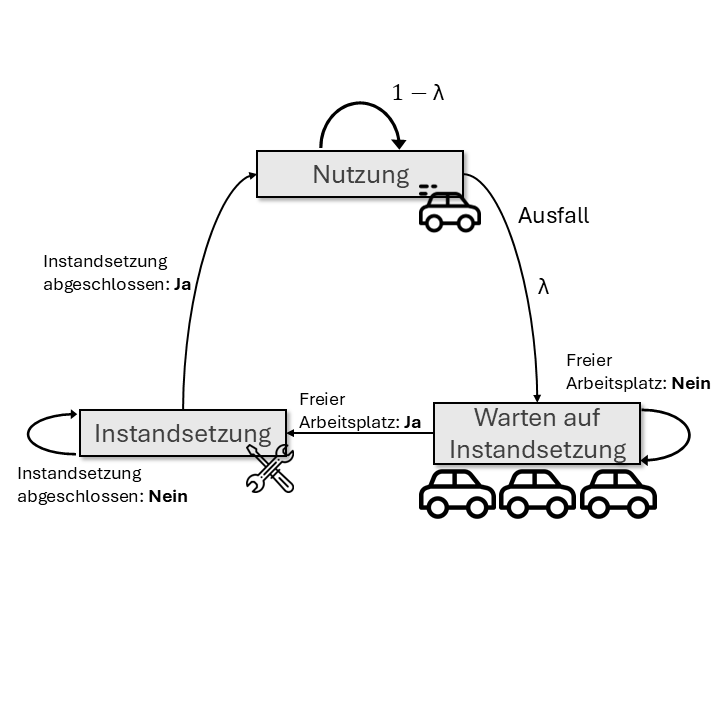
\includegraphics[width=\textwidth]{media/Simulationsmodell.png}
	\caption{
		Grundlegender Prozess innerhalb der Simulation. Fahrzeuge werden
		genutzt, fallen nach einiger Zeit aus und müssen dann instandgesetzt
		werden.
		}
	\label{fig:Simulationsmodell}
\end{figure}

Bereits in diesem vergleichsweise simplen Modell sind mehrere verschiedene Faktoren und KPI denkbar.

Beispiele für Faktoren:
\begin{itemize}
	\item Anzahl der Fahrzeuge
	\item Ausfallwahrscheinlichkeit der Fahrzeuge $\lambda$
	\item Höhe der Instandsetzungskapazitäten
	\item Reparaturrate der Fahrzeuge
\end{itemize}
Beispiele für KPI:
\begin{itemize}
	\item Anzahl einsatzbereiter Fahrzeuge
	\item Dauer von Reparaturen
	\item Länge der Warteschlangen
	\item Höhe der Wartezeiten
	\item Auslastung der Instandsetzungseinrichtungen
\end{itemize}

Für die vorliegende Implementierung des Simulationsmodells wurde das Python-Paket \emph{mesa} \cite{python-mesa-2020} genutzt.
Von den genannten Faktoren können die Anzahl der Fahrzeuge, die Höhe der Instandsetzungskapazitäten und die
Reparaturrate beeinflusst werden. Von den genannten KPI ist für die Anzahl einsatzbereiter Fahrzeuge
eine automatisierte Auswertung vorhanden.

Um eine möglichst optimale Konfiguration der Faktoren zu identifizieren, wird die Simulation 
mit vielen verschiedenen Konfigurationen durchgeführt und die dazugehörigen KPI ausgewertet.
Diese Methode ist auch unter dem Begriff \emph{Data Farming} bekannt \cite{8632383}.

In einer Simulation werden statt fester Werte oft Verteilungsfunktionen verwendet, aus denen Einflussgrößen abgeleitet werden. 
Aufgrund dieser Eigenschaft wird ein Simulationsmodell in der Regel mehrfach
mit gleichen Faktoren ausgeführt, um die stochastischen Effekte in den KPI zu beobachten und
um einzelne Ausreißer auszuschließen. 

Eine populäre Klassifizierung von Analysemodellen erfolgte durch Gartner \cite{Gartner} (vgl. Abbildung \ref{fig:gartner-modell}).
Diese Klassifizierung geht von vier Stufen von Analysemethoden aus, die anhand der Skalen \emph{Schwierigkeit} und \emph{Mehrwert} sortiert werden.
Beginnend bei niedriger Schwierigkeit und bei niedrigem Mehrwert bis hin zu hoher Schwierigkeit und hohem Mehrwert
handelt es sich dabei um:
\begin{enumerate}
	\item Deskriptive Analyse
	\item Diagnostische Analyse
	\item Prädiktive Analyse
	\item Präskriptive Analyse
\end{enumerate}

\begin{figure}
	\centering
	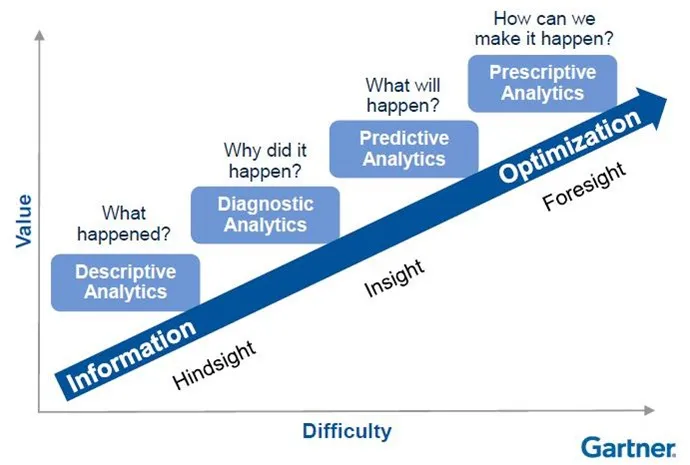
\includegraphics[width=\textwidth]{media/analytic-maturity.png}
	\caption{
		Das Gartner Modell schlägt eine Klassifizierung von Analysemodellen vor.
		Das hier dargestellte Simulationsmodell fällt in den Bereich der 
		präskriptiven Analyse. 
		}
	\label{fig:gartner-modell}
\end{figure}

Ein Simulationsmodell der hier vorliegenden Art fällt grundsätzlich in den Bereich der präskriptiven Analyse, 
da es nicht nur die Vorhersage zukünftiger Systemzustände erlaubt, sondern auch Faktoren identifiziert,
die verändert werden können, um einen bestimmten Zustand zu erreichen.

Ein Beispiel für eventuelle Nutzer einer Simulation wie der hier verwendeten, könnten 
Betreiber größerer Fahrzeugflotten (z.B. LKW oder Busse) sein. 
Gemäß Isermann \cite{Isermann_2011} belaufen sich bis zu 20 \% der laufenden Kosten beim Betrieb von Maschinen auf
die Instandhaltung bzw. Instandsetzung.
Fahrzeuge, die sich lange in Instandsetzung befinden, können in dieser Zeit keinen Mehrwert generieren.
Es besteht also ein Interesse daran, immer ausreichende Instandsetzungskapazitäten vorhalten zu können.
Da der Unterhalt derartiger Kapazitäten aber mit hohen Kosten verbunden ist, ist es von großem
Interesse, die \emph{optimale} Instandsetzungskapazität für eine gegebene Flotte zu identifizieren.

Der Bedarf an skalierbarer Infrastruktur zum Betrieb der Simulation ergibt sich daher wie folgt:
Bereits bei den vier oben aufgeführten Faktoren, mit denen das vorliegende Simulationsmodell betrieben werden könnte,
ergibt sich eine große Anzahl an Faktorkombinationen.
Angenommen jeder Faktor soll um fünf Stufen variiert werden. Dann ergeben sich daraus
$5^4 = 625$ Kombinationen. Aufgrund stochastischer Effekte empfiehlt es sich, jede einzelne
Kombination mehrfach zu wiederholen. Davon ausgehend, dass jede Kombination 20-mal wiederholt wird,
ergeben sich daraus schon $625 * 20 = 12.500$ Simulationsläufe. Bei einer angenommenen Laufzeit von ca. 10 Sekunden
pro Simulationslauf und rein serieller Ausführung ergibt sich daraus bereits eine Gesamtlaufzeit von
knapp 35 Stunden.

Bei Modellen für realistische Szenarien ist natürlich von mehr Faktoren und auch von einer höheren Zeit 
für einzelne Simulationsläufe auszugehen. Um einen vollständigen Simulationslauf möglichst schnell abzuschließen
und folglich auswertbare Ergebnisse zu erhalten, bietet es sich an, die Rechenlast zu verteilen.  

\subsection{Die Microservice-Architektur}
Nachdem im vorangegangenen Abschnitt die Motivation und die Funktionsprinzipien der Simulation erklärt wurden,
soll in diesem Abschnitt auf die für den Betrieb genutzte Microservice-Architektur Bezug genommen werden.


Grundlegend besteht die Microservice-Architektur aus sechs verschiedenen Services, deren Zusammenwirken
in Abbildung \ref{fig:microservice-architektur} dargestellt ist.

\begin{figure}
	\centering
	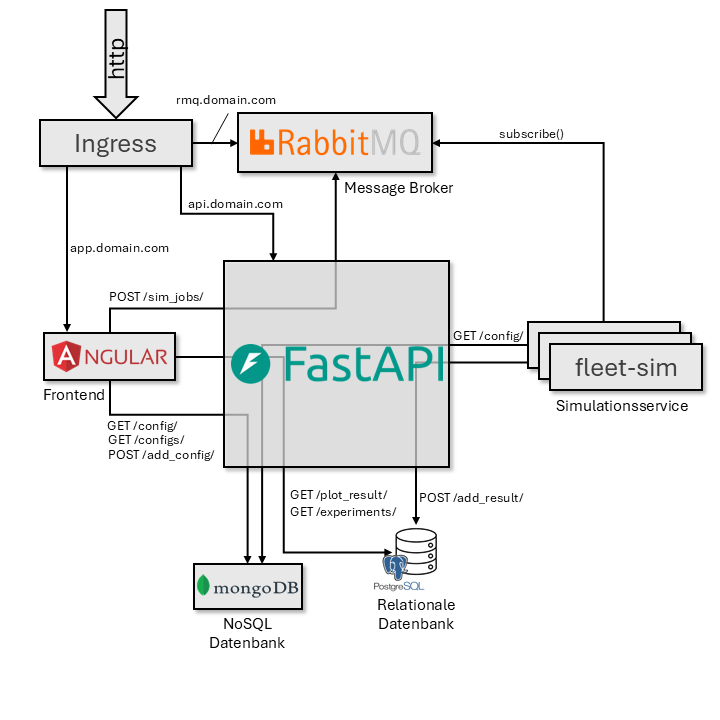
\includegraphics[width=\textwidth]{media/Microservice-Architektur.png}
	\caption{
		Eine Übersicht über die verwendete Microservice-Architektur.
		Details können dem Text entnommen werden.
		}
	\label{fig:microservice-architektur}
\end{figure}

Die Dateien, die zum Aufsetzen der Services verwendet wurden, sind unter
(\lstinline|https://github.com/patrick-meyer-1992/bachelorseminar|) \cite{Meyer_bachelorseminar}
verfügbar.

\subsubsection{Minikube}
Zum Aufsetzen des Clusters wurde \emph{Minikube} verwendet.
Minikube ist eine Anwendung, die genutzt werden kann, um mit vergleichsweise wenig Aufwand ein lokales
Kubernetes Cluster mit einem Node zu erstellen. Diese relativ einfache Konfiguration hat 
den Nachteil, dass Minikube lediglich für Test- und Entwicklungsaufgaben geeignet ist.
Für Produktivsysteme sollte eine andere Lösung gewählt werden (vgl. \ref{sec:Ausblick}). 

Zum Betrieb des Clusters verwendet Minikube eine virtuelle Maschine, innerhalb derer
alle Kubernetes Komponenten laufen. Dementsprechend ist eine der Voraussetzungen,
um Minikube zu nutzen auch die vorherige Installation einer Virtualisierungsanwendung.
Näheres kann der Minikube Dokumentation entnommen werden \cite{minikube}.

\subsubsection{FastAPI}
\label{sec:FastAPI}
FastAPI ist ein modernes, performantes Web-Framework, das genutzt werden kann, um \emph{Application-Programming-Interfaces} (API)
mit Python zu erstellen \cite{Ramirez_FastAPI}.

In diesem Fall wird es als zentrale Schnittstelle der Microservice-Architektur genutzt.
Anfragen an die Datenbanken (vgl. \ref{sec:Datenbanken})
über das Frontend (vgl. \ref{sec:Angular}) oder vom Simulationsservice (vgl. \ref{sec:Flottensimulation})
werden durch diese Schnittstelle angenommen, validiert, bearbeitet und beantwortet.
Gleiches gilt für die Befüllung der Job-Warteschlange (bzw. Message Queue) im Service
RabbitMQ (vgl. \ref{sec:RabbitMQ}), die über eine Anfrage seitens des Frontends an
FastAPI ausgelöst wird.

In der erstellten Microservice-Architektur wird das FastAPI-Deployment nur einfach repliziert,
da nicht zu erwarten ist, da in diesem Demonstrationsbeispiel (Proof-of-Concept) nicht von einer
großen Anzahl an Anfragen auszugehen ist. 
Die Anzahl der Replicas kann aber über ein einfaches Kommandozeilenargument angepasst werden, z.B.
(\lstinline|kubectl scale deployment fastapi-deployment --replicas=4|) 
falls das erforderlich sein sollte.

\subsubsection{Angular}
\label{sec:Angular}
Grundsätzlich ist es möglich, die Simulation vollständig über die Kommandozeile zu bedienen.
Da das Ziel einer solchen Simulation aber üblicherweise die Unterstützung von (nicht-technischen) 
Entscheidungsträgern ist, wurde ein Frontend entworfen, das eine Idee davon bieten soll, wie man Simulationsservices
einer breiteren Masse zur Verfügung stellen kann. Das Frontend basiert auf Angular,
einer Entwicklungsplattform zum Erstellen von Handy- und Desktop-Webanwendungen \cite{jain2014angularjs},
und ermöglicht das Konfigurieren, Starten und Auswerten von Simulationsläufen über eine interaktive Web-Oberfläche.
Ein Eindruck einer möglichen visuellen Auswertung kann Abbildung \ref{fig:ergebnis-plot} entnommen werden.

\begin{figure}
	\centering
	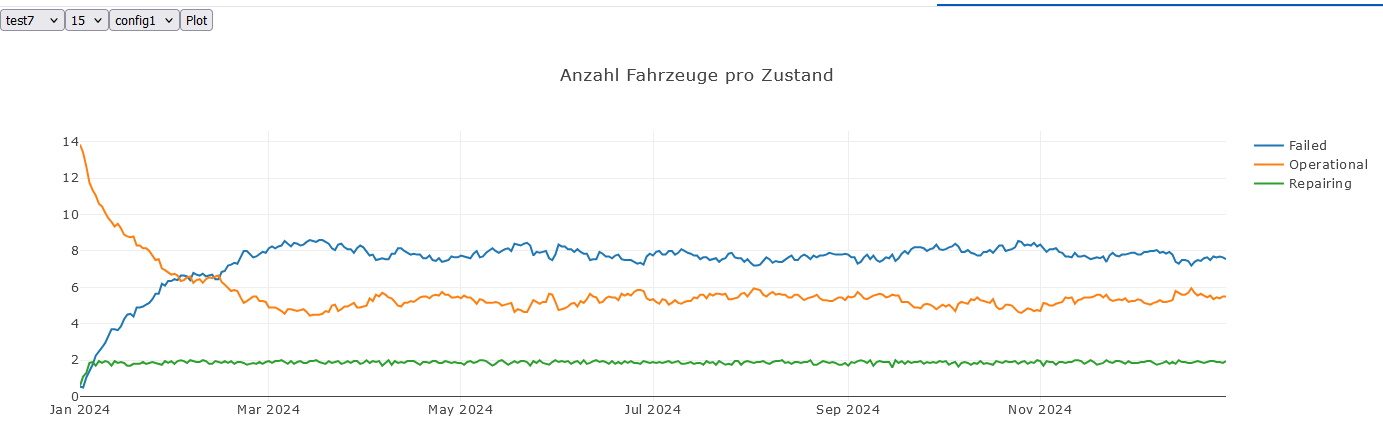
\includegraphics[width=\textwidth]{media/Ergebnisplot.png}
	\caption{
		Darstellung des Ergebnisses von einem Simulationslauf mit den eingestellten Faktoren.
		Zu sehen sind die Anzahl Fahrzeuge in den Zuständen „Ausgefallen“, „Einsatzbereit“ und „in Reparatur“	
		für jeden Tag des einjährigen Simulationszeitraums.
		}
	\label{fig:ergebnis-plot}
\end{figure}

\subsubsection{RabbitMQ}
\label{sec:RabbitMQ}
RabbitMQ ist ein Message- und Streaming-Broker \cite{RabbitMQ}. Es bildet eine Zwischenstation
zwischen Sender und Empfänger einer Nachricht. Das vereinfacht beispielsweise die Verteilung auf 
mehrere Empfänger, glättet Auslastungsspitzen und ermöglicht asynchrone Kommunikation zwischen
Sender und Empfänger. 

In der vorliegenden Microservice-Architektur wird RabbitMQ als Zwischenspeicher für
Simulationsaufträge genutzt. Das Frontend sendet für jeden einzelnen Simulationslauf
ein json-Objekt über FastAPI an RabbitMQ, wo jedes Objekt als ein Simulationsauftrag
in der Message Queue vorgehalten wird. Der Simulationsservice abonniert diese Message Queue,
wenn er gestartet wird und empfängt von dort einzeln seine Aufträge.

Dieses Vorgehen hat den Vorteil, dass Simulationsaufträge unabhängig von der Existenz
des Simulationsservices eingestellt werden können. Sobald der Simulationsservice gestartet
oder um weitere Replikationen ergänzt wird, beginnt die Bearbeitung der Aufträge durch den
bzw. die neuen Arbeiter.

\subsubsection{Datenbanken}
\label{sec:Datenbanken}
Zur persistenten Speicherung von Daten werden sowohl MongoDB als auch PostgreSQL verwendet.

MongoDB ist ein dokumentenorientiertes Datenbanksystem mit einem Fokus auf Skalierbarkeit und Flexibilität \cite{Bradshaw_2010}.
Dokumentenorientiert heißt in diesem Fall, dass die Daten nicht wie in einem relationalen
Datenbanksystem in Form von Tabellen gespeichert wird, sondern als Objekte in json-Notation.

In der Microservice-Architektur speichert MongoDB die Instandsetzungskonfigurationen,
die über das Frontend erstellt werden.
Eine Instandsetzungskonfiguration ist ein json-Objekt, das eine Liste von Instandsetzungseinrichtungen,
enthält. Diese enthalten wiederum eine Liste von Arbeitsplätzen, zu denen jeweils eine Liste
von Arbeitern gehört. 
Die Arbeiter enthalten Attribute, die ihre jeweilige Instandsetzungsgeschwindigkeit definieren.

Da eine Instandsetzungskonfiguration mitunter sehr komplex werden kann, war es wichtig,
dass einmal erstellte Konfiguration persistent gespeichert und auch wieder abrufbar und veränderbar sind.

Für die Speicherung der Simulationsergebnisse wird in diesem Szenario PostgreSQL als relationale Datenbank verwendet.

\subsubsection{Ingress}
Der Ingress-Controller hat die Aufgabe, Anfragen entsprechend des Hostnamens zu verteilen (vgl. \ref{sec:Ingress}).
In diesem Fall werden http-Anfragen gemäß der Subdomains \emph{app}, \emph{api}, \emph{rmq} an das
Frontend, den FastAPI-Service oder an den RabbitMQ-Service weitergeleitet. Um dieses Verhalten
in einer lokalen Umgebung zu ermöglichen, muss zusätzlich zum Cluster ein Weg eingerichtet werden,
um DNS-Anfragen an app.domain.com, api.domain.com und rmq.domain.com an die IP-Adresse des Clusters zu senden.
Das kann entweder durch das Aufsetzen eines DNS-Servers geschehen oder durch Anpassen der Datei 
\lstinline|/etc/hosts| unter Linux oder \lstinline|C:\Windows\system32\drivers\etc\hosts| unter Windows 11.

\subsubsection{Flottensimulation}
\label{sec:Flottensimulation}
Der Simulationsservice ist der Anteil der Microservice-Architektur, der den größten Anteil
der dort stattfindenden Berechnungen vornimmt und dementsprechend auch den größten Bedarf
an Rechenressourcen hat. Das ist insbesondere dann der Fall, wenn die Pods des Simulationsservice,
wie vorgesehen, vielfach repliziert werden.

Bei seinem Start abonniert jeder Pod unabhängig von den anderen die Job-Warteschlange von RabbitMQ.
Jeder Job enthält die konkreten Faktoren, mit denen der Simulationslauf durchgeführt werden soll.
Dazu gehört auch der Name der zugehörigen Instandsetzungskonfiguration. Aufgrund
dieses Namens wird die zu verwendende Instandsetzungskonfiguration über FastAPI
aus der MongoDB abgerufen.

Über einen Simulationszeitraum von einem Jahr wird für jeden Tag die Anzahl der Fahrzeuge
in den möglichen Zuständen (Einsatzbereit, Ausgefallen, in Reparatur) als KPI gespeichert.
Bei Abschluss der Simulation werden diese Ergebnisse ebenfalls über FastAPI in die 
PostgreSQL Datenbank geschrieben.

\section{Fazit}
Die erstellte Architektur konnte im Rahmen dieser Arbeit erfolgreich für die Konfiguration, Durchführung und grundsätzliche
Auswertung der Simulation genutzt werden. 
Kubernetes zeigte sich auch geeignet, um dem vorliegenden Anwendungsfall, nämlich die Skalierung des Simulationsservice,
zu unterstützen. 

Durch die Replikation der Pods kann die Rechenlast grundsätzlich effizient verteilt und 
die Gesamtlaufzeit der Simulationen deutlich reduziert werden 
(Auch wenn für diese Arbeit keine Hardware zur Verfügung stand, um das konkret zu testen).
Die Entkopplung der einzelnen Services ermöglicht zusätzlich die unabhängige Skalierbarkeit dieser.

Durch die Nutzung von FastAPI als zentrales Kommunikationselement ist es auch möglich, weitere Komponenten hinzuzufügen
oder bestehende zu verändern ohne, dass dafür alle anderen Komponenten angepasst werden müssen.
Es reicht stattdessen in der Regel, die Änderungen in FastAPI abzubilden.

RabbitMQ stellte sich als zielführende Lösung für die Verteilung von Simulationsaufträgen hinaus.
Eine Alternative, wie zum Beispiel die Verteilung der Simulationsaufträge nach dem Push-Prinzip an die Pods
hätte verschiedene Nachteile mit sich gebracht. Darunter die Tatsache, dass nur gerade aktive Pods
in der Lage gewesen wären, Aufträge entgegenzunehmen. Außerdem wären bei Fehler eines Pods alle
ihm zugeordneten Aufträge verloren gegangen.

Die Simulation an sich war zu Bestätigung des Funktionsprinzips gut geeignet,
müsste für einen realitätsnahen Einsatzzweck aber noch deutlich weiterentwickelt werden.
Schmeling und Dargatz \cite{Schmeling_Dargatz_2022}, Kap. 3 geben einen guten Überblick,
wie Kubernetes genutzt werden kann, um Anwendungsentwicklung zu unterstützen und zu beschleunigen.

Die Speicherung der Konfiguration der Instandsetzungseinrichtungen im json-Format stellte sich als 
angemessen für die Komplexität und Flexibilität eines derartigen Systems heraus. 
Vergleichbare Daten in klassischen relationalen Tabellenstrukturen zu speichern, wäre auch
möglich gewesen, könnte allerdings Limitationen bei der Flexibilität einbringen.
MongoDB als eine Anwendung, die insbesondere für die Speicherung und den Abruf von
Daten im json-Format gestaltet wurde, war für diesen Zweck dementsprechend gut geeignet.

Die Speicherung der Simulationsergebnisse in einer relationalen\linebreak PostgreSQL-Datenbank
erfolgte, da diese weniger komplex als die Konfigurationsdaten sind und weil
gängige Werkzeuge zur Datenanalyse gut mit tabellarisch organisierten zusammenwirken.
PostgreSQL als etabliertes Open-Source Werkzeug für relationale Datenbanken bot
hierfür eine leicht einzubindende Grundlage.

Angular als professionelles Werkzeug zur Erstellung von webbasierten Benutzeroberflächen,
ist geeignet, um einen zentralen Zugang für Nutzer zur Bedienung und Auswertung der Simulation zu bieten.
Für ein realistisches Einsatzszenario muss das Frontend noch um weitere Funktionen
und um grafische Aufbereitungen ergänzt werden.

Schließlich ist ein weiterer Vorteil die Unabhängigkeit von proprietären Anwendungen und die Möglichkeit, 
die gesamte Infrastruktur auf verschiedenen Plattformen (lokal oder in der Cloud) zu betreiben. 
Die Nutzung von Pods und Containern bringt zwar einen geringen Overhead mit sich,
der aber durch die Vorteile der Skalierbarkeit und Flexibilität ausgeglichen werden können.

Insgesamt hat sich Kubernetes als geeignetes Werkzeug für den gedachten Einsatzzweck erwiesen 
und bietet eine solide Grundlage für die weitere Entwicklung und den Betrieb der Simulationsanwendung.


\section{Limitationen}
Obwohl der für diese Arbeit geplante Anwendungsfall erfolgreich umgesetzt werden konnte,
gab es dennoch einige Limitationen in Bezug auf den Anwendungsfall an sich und auf
Kubernetes im Allgemeinen. Diese sollen in diesem Abschnitt diskutiert werden.

Die Skalierbarkeit des Simulationsservice mit Kubernetes auch über mehrere Rechner hinweg,
konnte aufgrund begrenzter Hardware nur eingeschränkt gezeigt werden. Ein alternativer Ansatz,
der mehrere virtuelle Maschinen verwendet, die jeweils einen Node abbilden, könnte 
für zukünftige Anwendungsfälle genutzt werden. Das war hier allerdings nicht realistisch,
da die zur Verfügung stehende Hardware nicht genug Rechen- und Speicherressourcen
für mehrere virtuelle Maschinen hatte.

Eine weitere Alternative wäre die Nutzung von kommerziellen Cloud-Anbietern.
Die wohl populärsten in diesem Zusammenhang sind Microsoft Azure,
Amazon Webservices und Google Kubernetes Engine. Alle drei Anbieter
ermöglichen den Betrieb von Kubernetes Clustern auf den von 
ihnen bereitgestellten Plattformen. Diese Dienstleistung
besteht aber entweder aus stark begrenzten Testversionen oder
ist mit hohen Kosten verbunden, weswegen sie für diese Arbeit nicht genutzt wurde.

Der Mangel an verfügbaren Rechen- und Speicherressourcen sorgte auch dafür,
dass die Microservice-Architektur keinem echten Stresstest unterzogen werden konnte.
Gerade im Bereich der verwendeten relationalen Datenbank könnte es bei vielen
parallelen Lese- und Schreibvorgängen schnell zu Leistungseinbußen kommen.
Die Replizierung relationaler Datenbanken unter Einhaltung des ACID-Prinzips
ist keine triviale Aufgabe und könnte für die weitere Ausgestaltung 
größere Herausforderungen mit sich bringen.

Da es sich in dieser Arbeit um das grundlegende Funktionsprinzip der Microservice-Architektur drehte,
wurde der Aspekt der Sicherheit an vielen Stellen vernachlässigt. Sollten die Services echten
Nutzern über das Internet zur Verfügung gestellt werden, müssten weitere Maßnahmen ergriffen werden.
Dazu gehört zunächst, dass die Kommunikation mit den http-Services verschlüsselt über https
stattfinden sollte. Zudem müsste gegebenenfalls ein Nutzerkonzept mit entsprechender
Authentisierung implementiert werden. Das gilt insbesondere dann, wenn sensible
Daten verarbeitet werden. Zusätzlich wurde keine Ausnahmebehandlung für fehlerhafte
Nutzereingaben und nur rudimentäres Eingabefeedback im Frontend integriert.
Generell fehlen für ein produktiv nutzbares System automatisierte Tests
aller Komponenten.

Die Skalierung des Simulationsservice fand in dieser Arbeit zwar mithilfe von Kubernetes
aber schlussendlich immer noch manuell statt, indem Kubernetes über die Kommandozeile angewiesen wurde
eine bestimmte Anzahl an Pods zu starten. Kubernetes bietet aber auch die Möglichkeit 
Services je nach Nutzlast automatisch zu skalieren. Für den vorliegenden 
Anwendungsfall war das nicht erforderlich, es könnte aber dennoch eine Verbesserung 
der Nutzbarkeit bewirken.

Abschließend bleibt zu erwähnen, dass Kubernetes zwar eine hohe Flexibilität bietet,
aber damit fast automatisch auch eine hohe Komplexität hat. Für große Anbieter von Onlinediensten
ist der Mehrwert durch diese Komplexität sicherlich vorhanden.
Für kleinere Unternehmen, die überlegen, Kubernetes zu verwenden, kann es sinnvoller sein,
alternative, simplere Methoden für die Serviceerbringung zu nutzen \cite{Pagani_2019}.

\section{Ausblick}
\label{sec:Ausblick}
Die hier beschriebene Microservice-Architektur war gedacht, um ein grundlegendes Prinzip
zu verdeutlichen. Einige weitere Einsatzmöglichkeiten von Kubernetes sind damit aber noch nicht ausgeschöpft 
und diese sollen in diesem Abschnitt diskutiert werden.

Zunächst sei angemerkt, dass Minikube zum Einrichten des Clusters für diesen Testfall
zwar völlig ausreichend war, in realistischen Szenarien aber durch andere Werkzeuge ersetzt werden sollte.
Für Kubernetes Cluster in Produktivumgebungen sind zum Beispiel \emph{Rancher}, \emph{OpenShift} oder \emph{Tanzu} als
gängige Lösungen verfügbar \cite{rancher}. Darüber hinaus bietet Kubernetes noch viele andere 
Anwendungsmöglichkeiten, wie zum Beispiel die Unterstützung von Entwicklern, um Software-Produkte
schneller von der Entwicklung bis zum produktiven Einsatz zu bringen \cite{Schmeling_Dargatz_2022}.

Bezüglich des Simulationsmodells sind je nach Anwendungsfall viele weitere Veränderungen denkbar.
Dazu gehören unter anderem die Berücksichtigung von Wartungsplänen und Nutzungsmustern, aber auch
die genauere Modellierung von Fahrzeugen und ihren Baugruppen. 
Zusätzlich könnte die Realitätsnähe der Simulation verbessert werden, indem die Option
implementiert wird, dass Faktoren sich auf der Zeitachse des Simulationslaufs dynamisch verändern.
Zum Beispiel ist es in einem realen Szenario sehr wahrscheinlich, dass Instandhaltungskapazitäten
sich im Laufe der Zeit verändern und nicht so bleiben, wie zu Beginn der Simulationszeit konfiguriert.

Abschließend bleibt festzuhalten, dass es sich bei Kubernetes zum Zeitpunkt des Erstellens dieser
Arbeit keineswegs um eine sich entwickelnde Technologie handelt, sondern um eine, die bereits
in vielen Bereichen von Forschung und Wirtschaft etabliert ist. In einer Umfrage der 
Cloud Native Computing Foundation von 2024 \cite{cncf} gaben 41 \% der befragten Unternehmen an,
bereits jetzt die meisten oder alle ihrer Anwendungen in einem Cloud-Umfeld zu betreiben und
80 \% gaben an, in den nächsten fünf Jahren die meisten oder alle ihrer neu entwickelten Anwendungen
auf der Cloud betreiben zu wollen. Durch den wachsenden Nutzerkreis wird auch mit Weiterentwicklungen
von Kubernetes in Bereichen der Bedienbarkeit und Standardisierung gerechnet \cite{emerging_trends}.
Erstere ist von großer Bedeutung, um Kubernetes einem größeren Feld an Entwicklern zugänglich
zu machen, während letztes einen wesentlichen Beitrag zur Flexibilität und Interoperabilität
leisten kann.

\section{Anhang}
\subsection{Selbstständigkeitserklärung}
Ich erkläre, dass ich die vorliegende Arbeit selbstständig und ohne fremde Hilfe verfasst habe.
Zitate aus anderen Quellen sind entsprechend gekennzeichnet.
Generative Künstliche Intelligenz (ChatGPT und GitHub Copilot) wurde in folgendem Umfang verwendet:
\begin{itemize}
	\item Suchen von Literatur
	\item Prüfung der Arbeit auf Rechtschreib- und Grammatikfehler
	\item Entwurf einer Gliederung (die nur unwesentlich übernommen wurde)
	\item Erstellung und Debugging von Code und Kubernetes-Skripten
\end{itemize}

\printbibliography
\end{document}